\chapter{Modernizing \texttt{next-common} And Storybook MCP Discovery}

\section{Context}

Because every micro-frontend application depends on next-common, any friction in its build pipeline, its component workshop (Storybook) or its runtime environment is amplified across the entire architecture.

During this internship, I was assigned three connected tasks on the \texttt{next-common} codebase:

\begin{enumerate}
    \item Upgrade the runtime toolchain to \textbf{Node.js 24} and \textbf{pnpm 10}, both in local development and in \acf{CI}.
    \item Upgrade \textbf{Storybook} to v10, adapt the configuration to its breaking changes, and explore the newly released \textbf{Storybook MCP server}.
    \item Integrate the \textbf{Storybook Performance Panel} addon so developers can detect performance regressions while writing stories.
\end{enumerate}

Although the three tasks were tracked as separate tickets, they form a coherent modernization effort: the Node/pnpm upgrade unblocks the Storybook upgrade, and the Storybook upgrade unlocks the ecosystem of v10-compatible addons including both the MCP server and the Performance Panel.

The following sections present these tasks in a logical order, explain the reasoning behind each decision and document the encountered migration issues.

\section{Task 1: Upgrading the Runtime Environment}

\subsection{Context and Motivation}

At the beginning of this task, the \texttt{next-common} repository was still based on \textbf{Node.js 20} and an older version of \textbf{pnpm}. As the shared frontend foundation used by multiple product teams, keeping the development environment aligned with the latest supported tooling was essential to ensure compatibility, maintainability, and long-term support.

The objective of this task was therefore to upgrade the project to \textbf{Node.js 24} and \textbf{pnpm 10}, while ensuring that the new runtime was consistently adopted across local development, continuous integration, and Docker-based environments.

\subsection{Implementation}

The migration affected the different parts of the development infrastructure.
\begin{table}[H]
\centering

\begin{tabular}{|p{4cm}|p{11cm}|}
\hline
\textbf{Component} & \textbf{Changes} \\
\hline

Package configuration &
Updated all \texttt{package.json} files to require Node.js~24 and pnpm~10 through the \texttt{engines} and \texttt{packageManager} fields. \\
\hline

Docker environment &
Rebased the development and testing Docker image on a Node.js~24 image and installed pnpm~10 during the build process. \\
\hline

GitHub Actions &
Updated CI workflows to execute builds and tests using Node.js~24 and pnpm~10 custom actions.\\
\hline

Documentation &
Updated the project documentation to reflect the new runtime prerequisites for contributors. \\
\hline

\end{tabular}
\caption{Main changes introduced during the runtime upgrade}
\label{tab:runtime-upgrade}
\end{table}

The Docker image used by the CI pipeline was also updated to rely on the new runtime environment, ensuring that local development and automated builds execute under identical conditions.

\subsection{Challenges}

Although the migration primarily involved infrastructure-level changes, it was relatively straightforward to implement. Nevertheless, the upgrade required several supporting adjustments to ensure compatibility across the development and CI environments. In particular, the project dependency lockfile had to be regenerated to reflect the updated package manager version, and portions of the CI configuration were revised to accommodate the new Node.js and pnpm runtime. These changes ensured consistent dependency resolution and reproducible builds across local development and automated pipelines. After these updates were applied, the entire build and test pipeline executed successfully without requiring any additional modifications, confirming the compatibility of the project with the upgraded runtime environment.

\subsection{Validation}

The upgraded environment was validated by executing the complete \ac{CI} pipeline, including package installation, project builds, automated tests and Storybook generation.

Successful execution of these workflows confirmed that the migration was fully compatible with the existing codebase while providing a standardized runtime environment based on Node.js~24 and pnpm~10.

\section{Task 2: Upgrading Storybook to v10 and Exploring the Storybook MCP Server}
\label{sec:storybook-upgrade}

\subsection{Context and Motivation}

Storybook plays a central role in the \texttt{next-common} ecosystem. Beyond serving as a component development environment, it acts as the primary platform for documenting reusable components, validating UI behavior, and performing visual regression testing before components are consumed by downstream applications.

The objective of this task was twofold:

\begin{itemize}
    \item Upgrade the existing Storybook installation to version 10 while ensuring compatibility with the existing component library and build pipeline.
    \item Explore the newly introduced Storybook \ac{MCP} server and evaluate how it can improve AI-assisted development workflows.
\end{itemize}

Besides benefiting from performance improvements and long-term maintenance, upgrading Storybook also enabled the adoption of newer addons and tooling that are only available for recent Storybook versions.

\subsection{Migration Strategy}

To minimize the migration risk, the upgrade was performed incrementally rather than replacing the entire configuration at once.

The migration followed four main steps:

\begin{enumerate}
    \item Inventorying all Storybook-related packages and addons currently used by the repository.
    \item Executing the official Storybook migration utility (\lstinline|pnpm dlx storybook@latest upgrade|) to automate the majority of the configuration changes.
    \item Reviewing the Storybook v10 migration guide and manually adapting the remaining breaking changes.
    \item Migrating deprecated configuration options to their Storybook v10 equivalents.
    \item Updating the preview configuration by introducing the strongly typed \lstinline|Preview| object and reorganizing global decorators.
    \item Validating the migration locally before executing the complete CI pipeline.
\end{enumerate}

This approach allowed automated transformations to be combined with manual verification, reducing the likelihood of regressions.

\subsection{Addons Migration}

Storybook addons were individually reviewed to verify their compatibility with version 10. This migration involved:

\begin{itemize}
    \item Replacing the deprecated \lstinline|@storybook/addon-essentials| package with its individual addons.
    \item Upgrading compatible addons such as Accessibility, Links, and Interactions.
    \item Updating internal addons to follow the new manager/preview registration API.
    \item Removing or replacing community addons that were no longer maintained or whose functionality had become part of Storybook itself.
\end{itemize}

Table~\ref{tab:addon-compat} summarizes the compatibility status of the different addons.

\begin{table}[H]
    \centering
    \begin{tabularx}{\textwidth}{|l|l|X|}
        \hline
        \textbf{Addon} & \textbf{Status} & \textbf{Action} \\
        \hline
        \texttt{@storybook/addon-essentials} & Deprecated &
        Split into individual addons. \\
        \hline
        \texttt{@storybook/addon-a11y} & Compatible &
        Updated to v10. \\
        \hline
        \texttt{@storybook/addon-links} & Compatible &
        Updated. \\
        \hline
        \texttt{@storybook/addon-interactions} & Compatible &
        Updated with minor API adaptations. \\
        \hline
        Internal custom addons & Required migration &
        Adapted to the new registration API. \\
        \hline
        Community addons & Mixed &
        Updated, replaced or removed depending on compatibility. \\
        \hline
    \end{tabularx}
    \caption{Storybook v10 addon compatibility}
    \label{tab:addon-compat}
\end{table}

\subsection{Migration challenges}

Although the official migration tool automated a significant portion of the upgrade, several issues required manual intervention.

The most important challenges encountered were:

\begin{itemize}
    \item Adapting documentation pages to the stricter MDX 3 parser.
    \item Updating Vite dependency pre-bundling to reduce cold startup times.
    \item Reducing the CI memory consumption during the static Storybook build.
    \item Reviewing and validating visual regression snapshots affected by changes in Storybook's default rendering behavior.
\end{itemize}

Resolving these issues ensured that both local development and CI builds remained stable after the migration.

\subsection{Exploring the Storybook MCP server}

Storybook 10 introduced a \textbf{Model Context Protocol (MCP) server}, an integration point that enables AI assistants, such as the one integrated into the Cursor IDE, to interact directly with Storybook. It allows these assistants to query the story index, retrieve story metadata, and reason about component APIs without relying on UI scraping or directly accessing the file system.

Exploring this capability was an integral part of this task, as it aligns with Rakuten's ``always-improve, always-advance'' principle. The MCP integration opens new possibilities for interacting with and understanding the component library, potentially improving developer productivity and making component discovery and usage more efficient.

\textbf{Configuration and Evaluation Steps:}

\begin{itemize}

    \item Registering the Storybook MCP server locally in the IDE's MCP configuration.

    \item Verifying that the assistant could list stories, retrieve their \texttt{args} and \texttt{argTypes}, and answer natural-language questions such as \emph{``Which stories in \texttt{next-common} render the \texttt{Button} in its \texttt{disabled} state?''} without requiring any source code to be manually provided.

    \item Using vibe coding to build a \texttt{/products} page that lists all available products in two scenarios: one with access to the Storybook MCP server and one without it, in order to compare the development experience and evaluate the benefits of MCP-assisted development.

\end{itemize}

\textbf{Observations:}

\begin{itemize}
    \item The MCP server is a genuine productivity multiplier for teams that already maintain a rich Storybook. It effectively turns the story catalog into a queryable knowledge base for AI assistants.
    \item Because it exposes structured story metadata rather than raw source code, it is a safer surface to grant an assistant than blanket repository access.
\end{itemize}

Figures~\ref{fig:product-no-mcp} and~\ref{fig:products-mcp} illustrate the results of implementing the \texttt{/products} page using vibe coding, first without access to the Storybook MCP server and then with MCP enabled. The comparison highlights the differences in the development experience and demonstrates how access to Storybook's component metadata can assist the AI assistant in understanding and reusing the available components.

\begin{figure}[H]
    \centering
    
\includegraphics[width=1\textwidth]{../assets/storybook_upgrade/products-no-mcp.png}
    \caption{\texttt{/products} page generated without access to the Storybook MCP server.}
    \label{fig:product-no-mcp}
\end{figure}

\begin{figure}[H]
    \centering
    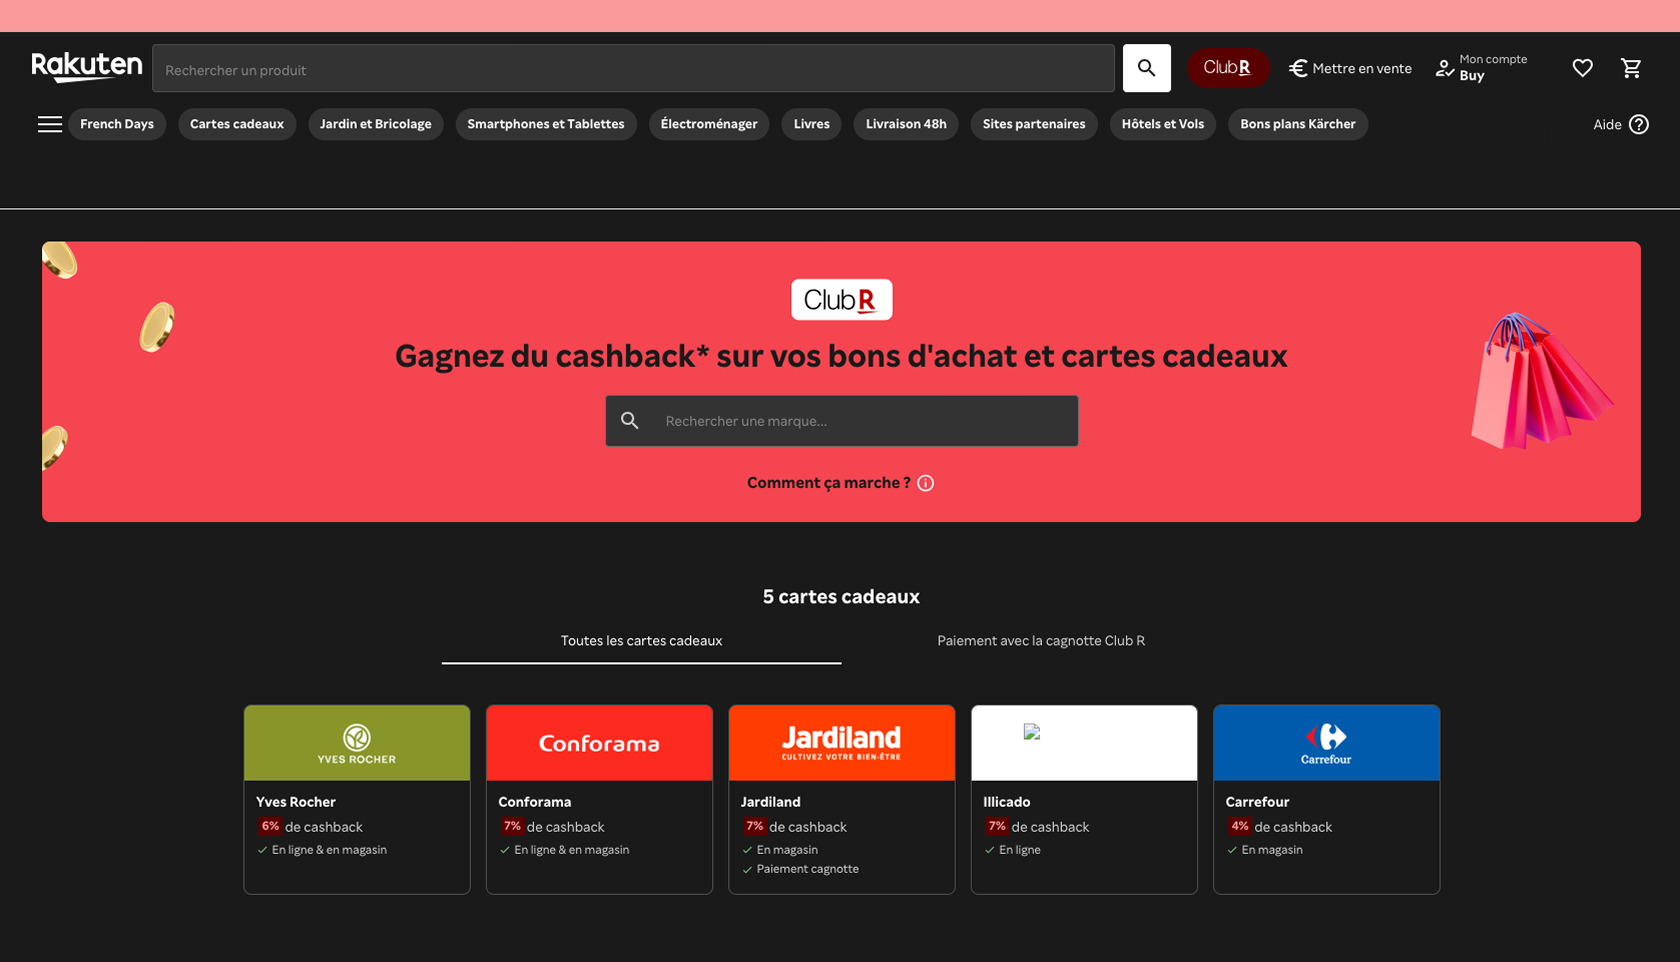
\includegraphics[width=1\textwidth]{../assets/storybook_upgrade/products-mcp.png}
    \caption{\texttt{/products} page generated with access to the Storybook MCP server.}
    \label{fig:products-mcp}
\end{figure}

\subsection{Validation}
\begin{itemize}
    \item Storybook dependencies were successfully upgraded to version 10.
    \item Development mode (\lstinline|pnpm book|) executed correctly.
    \item Static builds (\lstinline|pnpm book:build|) completed successfully both locally and in CI.
    \item Existing addons remained functional after migration.
    \item Shared components continued to render correctly, ensuring backward compatibility for downstream applications.
\end{itemize}

\section{Task 3 --- Adding the Storybook Performance Panel Addon}
\label{sec:task3-perf-panel}

\subsection{Motivation}

Performance regressions are notoriously hard to catch during code review. A component that renders in 40\,ms today may quietly grow to 200\,ms after a few refactors, because reviewers cannot easily observe render behavior from a diff. Once the regression lands, it becomes an incident-driven investigation.

The \textbf{Performance Panel} addon (\href{https://github.com/github/storybook-addon-performance-panel}{\texttt{@github-ui/storybook-addon-performance-panel}}) directly addresses this gap. It surfaces a live dashboard inside Storybook --- visible as a \textbf{Performance} panel next to Controls and Actions --- that displays render timings, re-render counts and other performance signals for the currently viewed story. Because every reusable component in \texttt{next-common} has at least one story, wiring the addon in gives us performance visibility everywhere, for free.

\subsection{Integration steps}

The integration was deliberately kept minimal and reversible.

\begin{enumerate}
    \item \textbf{Install the dependency.} Added \texttt{@github-ui/storybook-addon-performance-panel} as a \texttt{devDependency} in the Storybook workspace of \texttt{next-common}, then ran \texttt{pnpm install} to update the lockfile. Because this depends on Storybook 10, it could only be added \emph{after} Task 2 was merged --- which is why Task 2 had to come first in the timeline.
    \item \textbf{Register the addon in the manager.} Added the addon package name to the \texttt{addons} array in \texttt{.storybook/main.ts}, respecting the order convention (essential addons first, developer-experience addons after).
    \item \textbf{Compose the decorator in preview.} Imported the addon's decorator in \texttt{.storybook/preview.ts} and appended it to the global \texttt{decorators} array so it wraps every story without any per-story change.
    \item \textbf{Validate on a representative story.} Verified that the \textbf{Performance} panel appears in the Storybook toolbar and that switching between stories updates the metrics live. I validated this on a heavy, representative story (a data-dense product card grid) rather than a trivial one, because the addon's value shows most clearly on non-trivial trees.
\end{enumerate}

The full integration was under 15 lines of code.

\begin{figure}[h]
    \centering
    \fbox{\parbox{0.8\textwidth}{\centering \vspace{2cm} Placeholder for Figure~6 \vspace{2cm}}}
    \caption{The Performance panel visible in the Storybook UI for the \texttt{ProductCardGrid} story.}
    \label{fig:x6-perf-panel}
\end{figure}

\subsection{Acceptance criteria --- verification}

\begin{itemize}
    \item \texttt{@github-ui/storybook-addon-performance-panel} is added as a dependency in \texttt{next-common} Storybook. \textbf{Verified.}
    \item Addon is registered in \texttt{.storybook/main.ts}. \textbf{Verified.}
    \item Addon decorator is composed in \texttt{.storybook/preview.ts}. \textbf{Verified.}
    \item Storybook shows a \textbf{Performance} panel when viewing stories. \textbf{Verified} on Chrome and Edge (the browsers the addon documentation recommends for the full metric set).
    \item At least one representative story is validated with the panel working. \textbf{Verified} on \texttt{ProductCardGrid} and confirmed on two additional stories to make sure the wiring was not story-specific.
\end{itemize}

\subsection{Recommended usage}

I also added a short ``How to read the Performance panel'' note to the internal Storybook docs page, so contributors know:

\begin{itemize}
    \item Which metrics are meaningful for our stack (mount time, re-render count under prop churn).
    \item Which are noisy in a Storybook context and should not be treated as absolute (initial paint on a cold dev server).
    \item How to compare two branches by opening two Storybook tabs side by side.
\end{itemize}

\section{Cross-Cutting Challenges and How I Handled Them}

Beyond the per-task issues already documented, three cross-cutting challenges shaped how I approached the work:

\begin{itemize}
    \item \textbf{Coordinating three interdependent tickets.} Task 3 depends on Task 2, and Task 2 is significantly easier on Task 1's toolchain. I sequenced the PRs accordingly and kept them small enough to be reviewed independently, instead of bundling everything into a single unreviewable diff.
    \item \textbf{Not breaking downstream consumers.} \texttt{next-common} is consumed by other repositories. I audited its public exports before and after each upgrade and confirmed that no public API surface changed, so downstream consumers only had to bump the version.
    \item \textbf{Documenting for future contributors.} Every non-trivial migration step (MDX 3 strictness, \texttt{essentials} split, \texttt{packageManager} field, Docker base image change) was written down in the PR description and in the repository's \texttt{CONTRIBUTING.md}. The goal was to make the next Storybook or Node upgrade cheaper than this one.
\end{itemize}

\begin{figure}[h]
    \centering
    \fbox{\parbox{0.8\textwidth}{\centering \vspace{2cm} Placeholder for Figure~7 \vspace{2cm}}}
    \caption{PR overview showing the three sequential pull requests and their green CI status.}
    \label{fig:x7-prs}
\end{figure}

\section{Results and Impact}

The combined outcome of the three tasks:

\begin{itemize}
    \item \textbf{Modern runtime.} \texttt{next-common} now runs on Node 24 (Active LTS) and pnpm 10, consistent with the rest of the organization's repositories. CI images are rebuilt on the same baseline.
    \item \textbf{Modern component workshop.} Storybook 10 is live, with a faster dev server, cleaner configuration, an audited addon set, and no addon left behind.
    \item \textbf{New AI-assisted workflow surface.} Through the Storybook MCP server, AI assistants can now reason about \texttt{next-common} stories in a structured way, which is a genuine change in how the library can be consumed and extended.
    \item \textbf{Continuous performance visibility.} Every developer opening any story in \texttt{next-common} now sees a Performance panel by default, turning performance from an occasional audit into an ambient signal.
\end{itemize}

Together, these three changes shift \texttt{next-common} from a \emph{maintenance-friction} posture to an \emph{actively improving} posture --- which is precisely the theme of the branch this work targeted (\texttt{release/always-improve-always-advance}).

\section{Lessons Learned}

Reflecting on the internship work in this chapter, the main technical and methodological takeaways are:

\begin{itemize}
    \item \textbf{Sequence upgrades so that each unlocks the next.} Attempting the Storybook upgrade before the Node/pnpm upgrade would have wasted effort --- many v10 dependencies simply refuse to install on old runtimes. Ordering matters.
    \item \textbf{Prefer small, reviewable PRs on shared libraries.} A shared library is a high-leverage artifact; a broken commit has organization-wide blast radius. Splitting the work into three PRs made reviews faster and rollbacks safer.
    \item \textbf{Codemods are a starting point, not a substitute for reading the migration guide.} Storybook's codemod handled roughly 80\% of the mechanical work, but the remaining 20\% --- the parts that matter --- required reading the official guide and understanding the \emph{intent} behind each breaking change.
    \item \textbf{New protocol surfaces (MCP) are worth exploring early.} The Storybook MCP server is not yet mainstream, but adopting it early gave me a concrete view of how AI-assisted workflows can be grounded in real project metadata rather than raw source-code scraping.
    \item \textbf{Developer-experience tooling deserves the same rigor as production code.} The Performance Panel addon integration is only 15 lines of code, but choosing the right addon, validating it on a representative story, and documenting how to read its output is what turns those 15 lines into an actual team-level improvement.
\end{itemize}

\section{Conclusion}

This chapter documented three interconnected improvements to \texttt{next-common}: a runtime upgrade to Node 24 and pnpm 10, a Storybook upgrade to v10 with an exploration of its new MCP server, and the addition of the Storybook Performance Panel addon. Each task was small enough to ship independently, but together they constitute a coherent modernization of the front-end platform used across the organization.

The work aligned squarely with the branch it targeted --- \texttt{release/always-improve-always-advance} --- and left \texttt{next-common} on a foundation that is faster to iterate on, safer to maintain, and more open to AI-assisted development workflows for the teams that will inherit it.

\clearpage
